\begin{frame}{introduction}{vision \& mission}
    \vspace{-7mm}
    \begin{columns}
    \column{.65\linewidth}
        \begin{itemize}
            \item<1->   \textbf{vision}
            \begin{itemize}
                \item \textbf{democratization} of 
                    \begin{itemize}
                        \item music making
                        \item music education
                        \item music discovery
                    \end{itemize}
                \smallskip
                \item<2->[$\Rightarrow$] through \textbf{machine understanding of music} 
                    \begin{itemize}
                        \item   musically meaningful discovery \& processing
                        \item   musically meaningful / controllable generation
                        \item   musically intelligent ai tutors
                    \end{itemize}
            \end{itemize}
        \smallskip
        \item<3->   \textbf{mission}
            \begin{itemize}
                \item   create new technologies transforming and enhancing how we \textit{make, produce, perform, discover,} and \textit{consume music}
                \item   advance the field of AI for audio/music through \textit{knowledge-driven machine learning}
            \end{itemize}
        \end{itemize}
    \column{.35\linewidth}
        \only<2->{
        \begin{figure}
            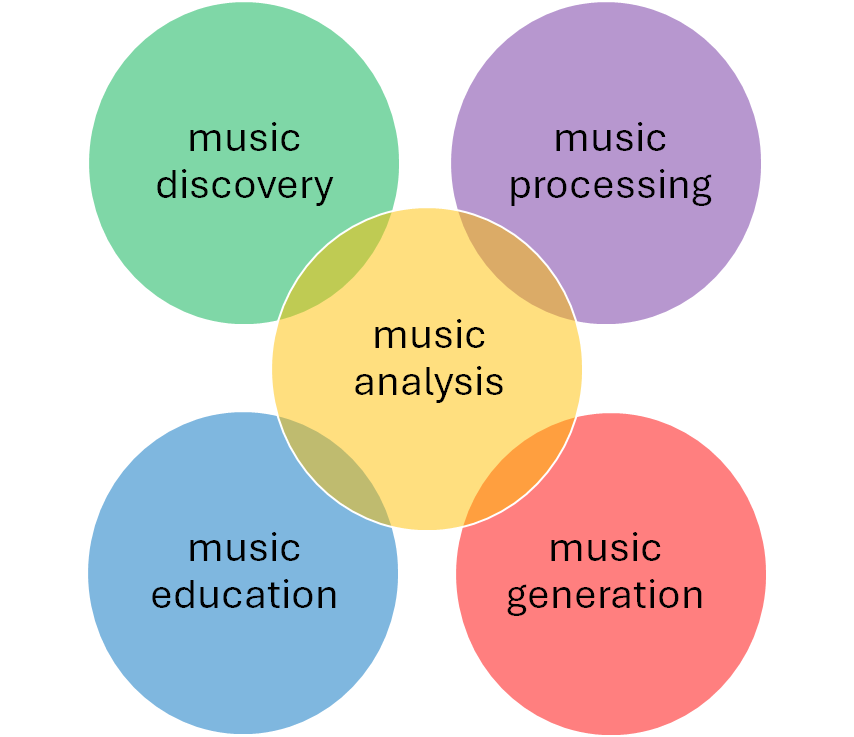
\includegraphics[width=1.2\columnwidth]{music_analysis}
        \end{figure}
        }
    \end{columns}
\end{frame}

\begin{frame}{introduction}{research focus (tasks)}
    \vspace{-9mm}
    \begin{columns}
    \column{.6\linewidth}
    \begin{itemize}
        \item   \textbf{music analysis} 
            \begin{itemize}
                \item   music/audio \textit{classification}
                    \begin{itemize}
                        \item genre/events \cite{burred_hierarchical_2004, hung_low-resource_2023}
                        \item instruments \cite{gururani_semi-supervised_2021, chen_music_2023, ding_audio_2023}
                        \item tagging \cite{ding_audio_2023, ding_embedding_2024, ma_music_2024}
                        \item emotion \cite{watcharasupat_uncertainty_2025}
                        %\item pedestrians \cite{seshadri_asped_2024, han_understanding_2024}
                    \end{itemize}
                \item   music \textit{transcription}
                    \begin{itemize}
                        \item drum transcription \cite{wu_review_2018}
                        \item chord detection \cite{zhou_chord_2015}
                        \item pitch tracking \cite{lerch_introduction_2023}
                    \end{itemize}
                \item   music \textit{performance analysis} \cite{lerch_software-based_2009, pati_assessment_2018}
            \end{itemize}
         \smallskip
         \item<2->  \textbf{music processing}
            \begin{itemize}
                \item   music source separation \cite{hung_multi-task_2020, watcharasupat_generalized_2024, watcharasupat_stem-agnostic_2024}
            \end{itemize}
         \smallskip
         \item<3->  \textbf{sound and music generation}
            \begin{itemize}
                %\item   controllability \cite{pati_attribute-based_2020}
                \item   evaluation \cite{yang_evaluation_2020, pati_is_2021, watcharasupat_latte_2022, vinay_evaluating_2022}
            \end{itemize}
    \end{itemize}
    \column{.4\linewidth}
    \begin{figure}
        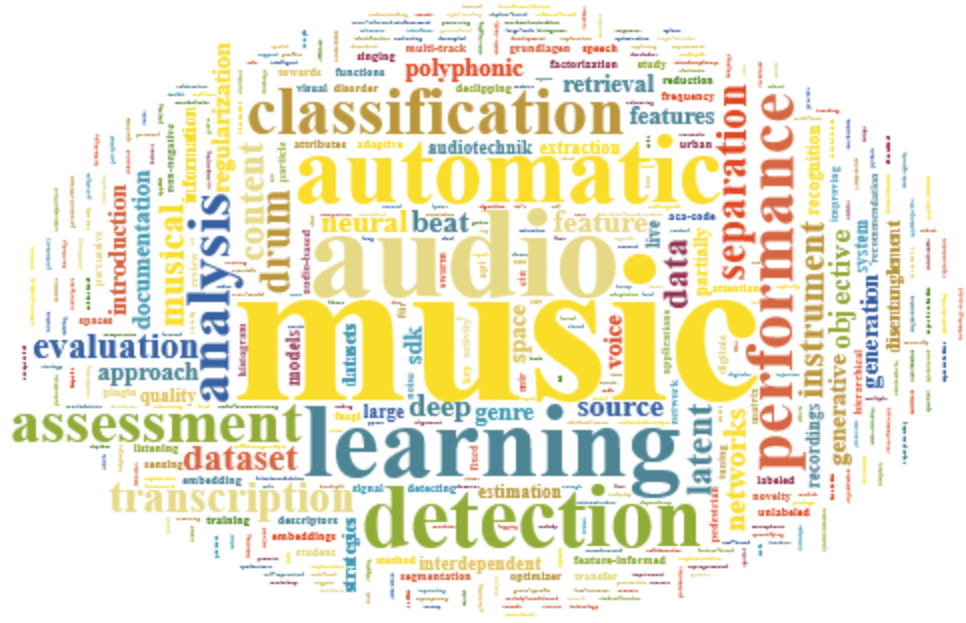
\includegraphics[width=\columnwidth]{research_cloud}
    \end{figure}
    \end{columns}
    \vspace{-25mm}
    \begin{flushright}
        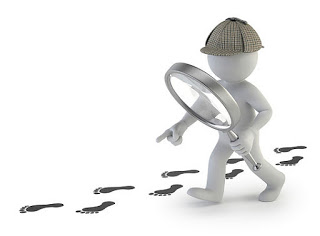
\includegraphics[scale=.25]{forensics}
    \end{flushright}
\end{frame}
        
                
                %\begin{frame}{introduction}{music information retrieval}
        %\end{frame}
        %\begin{frame}{introduction}{content in audio signals}
             %\begin{columns}
             %\column{.4\textwidth}
                %examples for audio signal content
                %\begin{itemize}
                    %\item   \textbf{speech}
                        %\begin{itemize}
                            %\item   text information
                            %\item   speaker
                            %\item   recording environment
                            %\item   \dots
                        %\end{itemize}
                    %\item   \textbf{music}
                        %\begin{itemize}
                            %\item   melody
                            %\item   harmony
                            %\item   structure
                            %\item   instruments
                            %\item   mood
                            %\item   genre
                            %\item   \dots
                        %\end{itemize}
                %\end{itemize}
             %\column{.6\textwidth}
                %\figwithmatlab{Waveform}
                %\begin{center}
                %\begin{tabular}{p{.3\columnwidth}p{.3\columnwidth}p{.3\columnwidth}}
                    %\includeaudio{excerpt_speech} & \includeaudio{excerpt_stringquartet} & \includeaudio{excerpt_pop}
                %\end{tabular}
                %\end{center}
             %\end{columns}
        %\end{frame}
%
        %\begin{frame}{introduction}{audio content analysis --- research fields}
            %\vspace{-7mm}
            %\begin{columns}
            %\column{.7\textwidth}
            %\begin{itemize}
                %\item   \textbf{speech} analysis
                    %\begin{itemize}
                        %\item   speech recognition
                        %\item   speech emotion recognition, \ldots
                    %\end{itemize}
                %\smallskip
                %\item<2->   \textbf{urban sound} analysis
                    %\begin{itemize}
                        %\item   noise pollution monitoring
                        %\item   audio surveillance, \ldots
                    %\end{itemize}
                %\smallskip
                %\item<3->   \textbf{industrial sound} analysis
                    %\begin{itemize}
                        %\item   monitoring the state of mechanical devices
                        %\item   monitoring the health of livestock, \ldots
                    %\end{itemize}
                %\smallskip
                %\item<4->   \only<5->{\textcolor{gtgold}}{\textbf{musical audio} analysis}
                    %\begin{itemize}
                        %\item   music transcription
                        %\item   music classification, \ldots
                    %\end{itemize}
            %\end{itemize}
            %\column{.3\linewidth}
                %\begin{figure}%
                    %\includegraphics[width=\columnwidth]{ai_w_headphones}%
                %\end{figure}
            %\end{columns}
        %\end{frame}
        %
        %\begin{frame}{introduction}{musical audio vs.\ other audio}
            %\vspace{-3mm}
            %\begin{columns}
            %\column{.7\textwidth}
            %\textbf{music} \ldots
            %\begin{itemize}
                %\item   is a \textbf{wide band} signal(\emph{unlike many other audio signals})
                %\item<2->   comprises both \textbf{tonal and noise} components(\emph{like most audio signals})
                %\item<3->   combines \textbf{multiple sound sources}(\emph{unlike speech, like urban sound})
                %\item<4->   is a \textbf{poly-timbral} mixture(\emph{nlike industrial sound})
                %\item<5->  sources are \textbf{harmonically related and synchronous} (\emph{unlike other multi-source signals})
                %\item<6->   has a highly structured \textbf{sequential} language that is \textbf{abstract} (\emph{unlike speech})
            %\end{itemize}
            %\column{.3\linewidth}
                %\begin{figure}%
                    %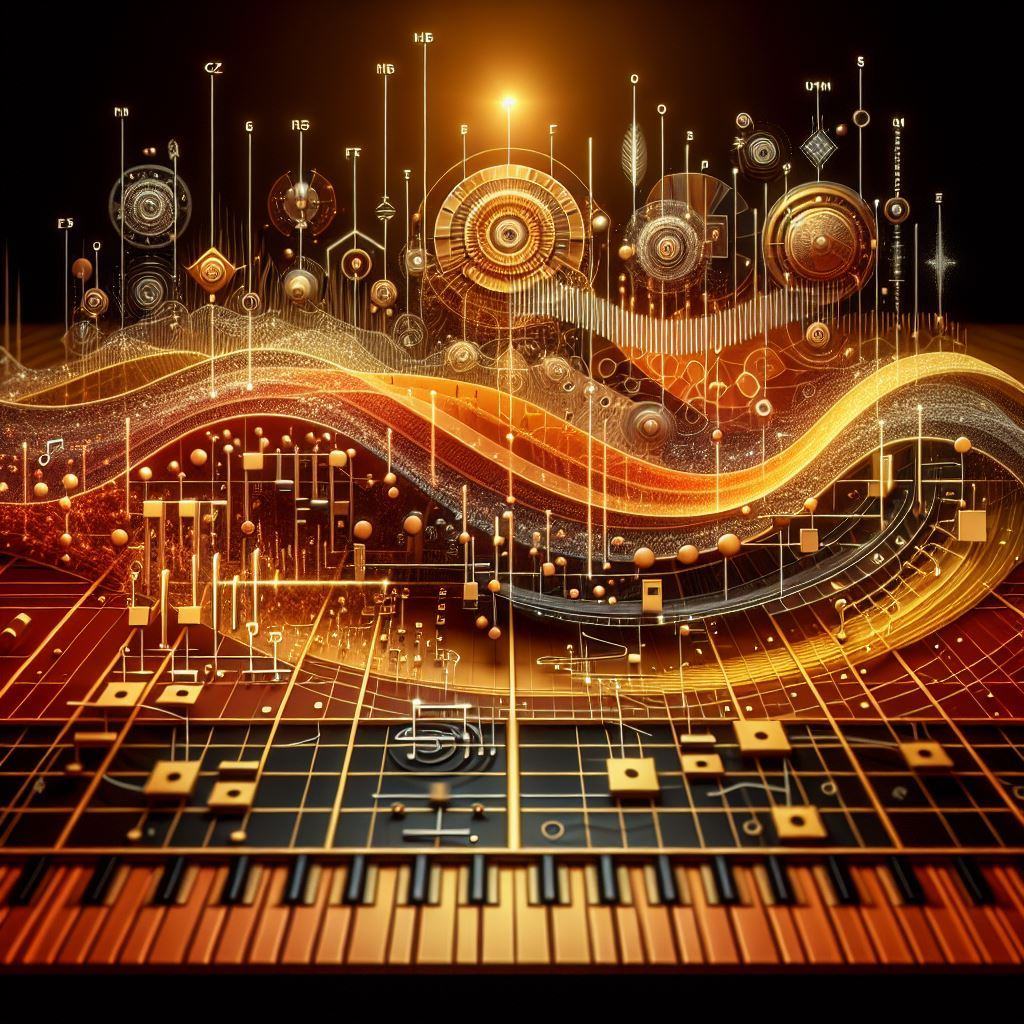
\includegraphics[width=\columnwidth]{music}%
                %\end{figure}
            %\end{columns}
        %\end{frame}
        %
       %\begin{frame}{introduction}{use cases}
            %\vspace{-3mm}
            %\begin{columns}
            %\column{.7\textwidth}
            %\begin{itemize}
                %\item	\textbf{music browsing and music discovery} 
                    %\begin{itemize}
                        %\item   search \& retrieval, recommendation, similarity, interfaces (e.g., QBH)
                    %\end{itemize}
                %\smallskip
                %\item<2->	\textbf{music consumption} 
                    %\begin{itemize}
                        %\item   creative music listening
                    %\end{itemize}
                %\smallskip
                %\item<3->	 \textbf{music production}
                    %\begin{itemize}
                        %\item   adaptive parametrization, enhancements of creative process
                    %\end{itemize}
                %\smallskip
                %\item<4->	\textbf{music education}
                    %\begin{itemize}
                        %\item   musically intelligent software tutoring
                    %\end{itemize}
                %\smallskip
                %\item<5->	\textbf{generative music}
                    %\begin{itemize}
                        %\item   interactive soundtracks (games, video)
                    %\end{itemize}
            %\end{itemize}
            %\column{.3\linewidth}
                %\begin{figure}%
                    %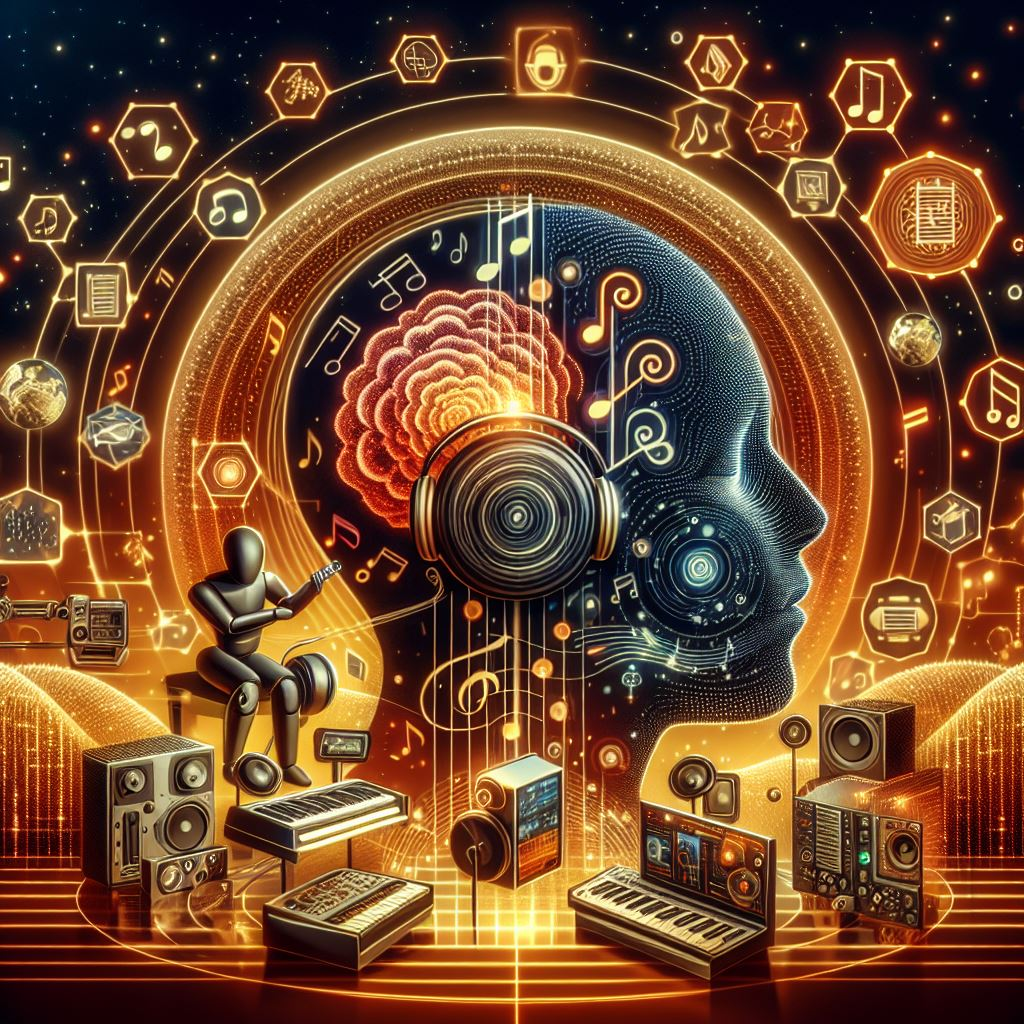
\includegraphics[width=\columnwidth]{musictech-apps}%
                %\end{figure}
            %\end{columns}
            %
        %\end{frame}
         
        
%\begin{frame}{musical communication}{chain of musical communication}
      %\vspace{-3mm}
        %\begin{figure}
                %\centering
                %\begin{picture}(140,35)
                    %%boxes
                    %%\only<1>{\color{gtgold}
                    %{\put(0,30){\ovalbox{\footnotesize{\parbox{20mm}{\vspace{2mm}\centering{\only<1>{\textcolor{gtgold}}{composition}}}}}}}
                    %%}
                    %\put(30,30){\ovalbox{\footnotesize{\parbox{20mm}{\vspace{2mm}\centering{\only<2>{\textcolor{gtgold}}{performance}}}}}}
                    %\put(60,30){\ovalbox{\footnotesize{\parbox{20mm}{\vspace{2mm}\centering{\only<3>{\textcolor{gtgold}}{production}}}}}}
                    %\put(90,30){\ovalbox{\footnotesize{\parbox{20mm}{\vspace{2mm}\centering{\only<4>{\textcolor{gtgold}}{distribution}}}}}}
                    %\put(120,30){\ovalbox{\footnotesize{\parbox{20mm}{\vspace{2mm}\centering{\only<4>{\textcolor{gtgold}}{consumption}}}}}}
        %
                    %% horizontal
                    %\put(22.4,30.6){\vector(1,0){7.8}}
                    %\put(52.4,30.6){\vector(1,0){7.8}}
                    %\put(82.4,30.6){\vector(1,0){7.8}}
                    %\put(112.4,30.6){\vector(1,0){7.8}}
                %\end{picture}
            %\end{figure}
            %\vspace{-27mm}
    %\begin{itemize}
        %\item<1-> \textbf{creation of musical ideas} (``score'')
            %\begin{itemize}
                %\item   defines style and idea
            %\end{itemize}
        %\smallskip
        %\item<2-> \textbf{realization of musical ideas} into acoustical rendition 
            %\begin{itemize}
                %\item   interpretation, modification, addition, and dismissal of score information
                %\item   unique acoustic representation of score
            %\end{itemize}
        %\smallskip
        %\item<3-> \textbf{recording, mixing, and editing} (in case of record media)
            %\begin{itemize}
                %\item   editing and splicing of recorded data; timbre, equalization choices
                %\item   not separable from performance in a recording
            %\end{itemize}
        %\smallskip
        %\item<4-> \textbf{distribution \& listening}
            %\begin{itemize}
                %\item   music recommendation and discovery
            %\end{itemize}
    %\end{itemize}
    %\inserticon{directions}
%\end{frame}


